\documentclass[]{article}
\usepackage{lmodern}
\usepackage{amssymb,amsmath}
\usepackage{ifxetex,ifluatex}
\usepackage{fixltx2e} % provides \textsubscript
\ifnum 0\ifxetex 1\fi\ifluatex 1\fi=0 % if pdftex
  \usepackage[T1]{fontenc}
  \usepackage[utf8]{inputenc}
\else % if luatex or xelatex
  \ifxetex
    \usepackage{mathspec}
  \else
    \usepackage{fontspec}
  \fi
  \defaultfontfeatures{Ligatures=TeX,Scale=MatchLowercase}
\fi
% use upquote if available, for straight quotes in verbatim environments
\IfFileExists{upquote.sty}{\usepackage{upquote}}{}
% use microtype if available
\IfFileExists{microtype.sty}{%
\usepackage{microtype}
\UseMicrotypeSet[protrusion]{basicmath} % disable protrusion for tt fonts
}{}
\usepackage{hyperref}
\hypersetup{unicode=true,
            pdfborder={0 0 0},
            breaklinks=true}
\urlstyle{same}  % don't use monospace font for urls
\usepackage{graphicx,grffile}
\makeatletter
\def\maxwidth{\ifdim\Gin@nat@width>\linewidth\linewidth\else\Gin@nat@width\fi}
\def\maxheight{\ifdim\Gin@nat@height>\textheight\textheight\else\Gin@nat@height\fi}
\makeatother
% Scale images if necessary, so that they will not overflow the page
% margins by default, and it is still possible to overwrite the defaults
% using explicit options in \includegraphics[width, height, ...]{}
\setkeys{Gin}{width=\maxwidth,height=\maxheight,keepaspectratio}
\IfFileExists{parskip.sty}{%
\usepackage{parskip}
}{% else
\setlength{\parindent}{0pt}
\setlength{\parskip}{6pt plus 2pt minus 1pt}
}
\setlength{\emergencystretch}{3em}  % prevent overfull lines
\providecommand{\tightlist}{%
  \setlength{\itemsep}{0pt}\setlength{\parskip}{0pt}}
\setcounter{secnumdepth}{0}
% Redefines (sub)paragraphs to behave more like sections
\ifx\paragraph\undefined\else
\let\oldparagraph\paragraph
\renewcommand{\paragraph}[1]{\oldparagraph{#1}\mbox{}}
\fi
\ifx\subparagraph\undefined\else
\let\oldsubparagraph\subparagraph
\renewcommand{\subparagraph}[1]{\oldsubparagraph{#1}\mbox{}}
\fi
			MathJax.Hub.Config({
				showProcessingMessages: false,
				messageStyle: "none",
				TeX: { equationNumbers: {autoNumber: "all"} },
				extensions: ["tex2jax.js"],
				jax: ["input/TeX", "output/HTML-CSS"],
				tex2jax: {
					inlineMath: [ ['$','$'] ],
					displayMath: [ ['$$','$$'] ],
					processEscapes: true
				},
		        SVG: { linebreaks: { automatic: true } },
				"HTML-CSS": { availableFonts: ["TeX"] }
			});
/*
			MathJax.Hub.Config({
		        TeX: { noErrors: { disabled: true } }
			});
*/

\date{}

\begin{document}

\section{Charges in a conductor and Gauss's
Law}\label{charges-in-a-conductor-and-gausss-law}

Developed by Larry Engelhardt

In this activity, students simulate and visualize the motion of excess
charges in a conductor (both a sphere and a cube) in three-dimensional
space, without any external electric field. Students also compute the
electric field from the conductor and discuss the results in the
following three regimes: (1) Far from the conductor, (2) Close to the
conductor, and (3) Inside the conductor.

Note: Student-facing documents that have been used with students in a
lab setting are provided under the ``Code'' tab as ``Additional
Resources''.

\begin{description}
\tightlist
\item[Course Context]
First Year and Beyond the First Year Electricity \& Magnetism
\item[Learning Objectives]
Students will be able to:
\end{description}

\begin{itemize}
\tightlist
\item
  Calculate the number of electrons for a total charge (\textbf{Exercise
  1})
\item
  Observe and describe both the \emph{approach} to equilibrium (the
  ``transient'' dynamics) and the final arrangement for charges in a
  conductor {[}\textbf{Exercises 2 (sphere); and 7, 8, and 9 (cube)}{]}
\item
  Write a computer function that will compute the net electric field
  from a system of system of charged particles (\textbf{Exercise 3})
\item
  Validate their numerical E-field results {[}\textbf{Exercises 4
  (sphere) and 10 (cube)}{]}
\item
  Test Gauss' Law numerically, and describe the results in the vicinity
  of a conductor {[}\textbf{Exercises 5 (close to a sphere), 6 (inside a
  sphere), 11 (close to a cube), and 12 (inside a cube)}{]}
\end{itemize}

\subsection{Instructor's Guide}\label{instructors-guide}

\textbf{Overview:}

A huge part of this activity is \textbf{\emph{seeing}} the charges repel
from one another, end up on the surface of the conductor, and finally
reach equilibrium. Upon seeing this for the first time, the students
said an audible, ``whoa''. After the ``whoa'' students then also do some
\textbf{\emph{coding}} and use their code to do some
\textbf{\emph{analysis}} and \textbf{\emph{interpretation}}.

\textbf{Context:}

I have used this Exercise Set in my introductory calculus-based E\&M
course as part of a 3-hour lab activity. During this 3-hour lab, I have
started with a brief lecture in which we talk about both (1) unit
vectors (specifically the meaning of the \(\hat{r}\) vector), which is
needed in order to calculate both \(\vec{E}\) and \(\vec{F}\); and (2)
the lines of code that they will be given. The students typically spent
about 2.5 hours working on this (in pairs), and they were given a quiz
at the end of the lab time.

\textbf{Prerequisites:}

Before doing this activity, the students had already been exposed to:

\begin{enumerate}
\def\labelenumi{\arabic{enumi}.}
\tightlist
\item
  Coulomb's Law
\item
  Gauss's Law
\item
  Any excess charge will reside on the surface of a conductor
\end{enumerate}

Coulomb's Law is certainly a prerequisite for this activity; it is used
throughout. I would also consider Gauss's Law to be a prerequisite,
since it provides both (A) a nice grounds for comparison of numerical
data and (B) allows the opportunity to \emph{refine} a students
understanding of Gauss's Law; namely, Gauss's Law is not very useful
outside of a cube, since it lacks the symmetry that would be necessary
in order for us to calculate \(E\) from Gauss's Law. Item 3 (that any
excess charge will reside on the surface of a conductor) wouldn't need
to be introduced before this activity. It could be ``discovered'' as a
part of this ``computational experiment''. I am not sure which order
would work better here, but I plan to try it the other way next time
(allowing it to be discovered during the activity).

\textbf{Results:}

The numerical results from this simulation offer the following insights
that are typically not appreciated when using strictly analytical
methods:

\begin{enumerate}
\def\labelenumi{\arabic{enumi}.}
\tightlist
\item
  When we are relatively far from a charge distribution, that charge
  distribution \textbf{\emph{always}} looks like a point charge at the
  center of the distribution, even if the charge distribution is spread
  out on the surface of a cube.
\item
  We are able to observe ``experimentally'' that the electric field does
  indeed go to zero inside of a conductor. Note that with a finite
  number of charges, \(E\) is not \emph{exactly} zero, but it is orders
  of magnitude smaller than the value of \(E\) outside of the conductor.
\item
  We can verify that Gauss's Law does in fact ``work'' for a spherical
  conductor; namely that the sphere ``looks like'' a point charge at the
  origin when we are outside of the sphere.
\item
  We can experience the \emph{limitations} of Gauss's Law. Namely,
  Gauss's Law is not very useful outside of the cube, since it lacks the
  symmetry of the sphere. So the cube does \textbf{not} look like a
  point charge at the origin (unless you are very far away from the
  cube).
\end{enumerate}

For introductory E\&M, I only ask the students to compute \(E\) at
specific locations, but for upper-level E\&M, it would be very
appropriate to ask the students to write a \emph{loop} in order to
compute the value of \(E\) for many values of \(r\) (the distance from
the origin) and to plot the results.

\textbf{Tips:}

Be aware that the electric field will not \emph{perfectly} cancel inside
of the simulated conductor since a finite number of charges are being
used. In Exercise 6, the students are asked to use a value of \(r\) that
is located reasonably far inside of the conductor, which will provide
good cancellation, such that the net electric field will be quite close
to zero. If the students experiment with different positions within the
conductor, they are likely to see that the electric field is not zero as
they get close to the surface. The reason is that they are able to
``see'' the discrete nature of the charges when they get close to the
surface, whereas far from the surface the charges appear continuous.

This code will run and display quite quickly using glowscript,
especially in the Chrome web browser. If you are familiar with Jupyter
Notebooks, you can also run this code in Jupyter. However, it will run
much slower in Jupyter.

\textbf{Algorithm:}

(See
\url{http://www.compadre.org/PICUP/resources/Numerical-Integration/} for
additional details about algorithms for computing dynamics.)

For the charges in a \emph{spherical} conductor, the algorithm that is
used doesn't particularly matter; the Euler of Euler-Cromer algorithm
work fine. In the rectangular (or cubic) conductor, there is an
interesting ``twist''. Before describing the twist, I should note that
\textbf{I HAVE NEVER POINTED THE FOLLOWING ISSUE OUT TO THE STUDENTS,
AND THEY HAVE NEVER NOTICED OR ASKED ABOUT THIS}.

Here is the twist:

When two or more charges end up together on the edge of the cube, a
first order algorithm (Euler or Euler-Cromer) is not stable and will
quickly ``blow up''. One could instead use a higher-order algorithm
(velocity Verlet of Runge-Kutta), but I didn't want to add extra code
that would distract students from what they were doing. So instead, I
treated the charges in the ``large friction limit,' where the force is
\textbf{not} used to update the velocity according to Newton's 2nd Law,
\[\frac{\Delta \vec{v}}{\Delta t} = \frac{\vec{F}_{net}}{m}.\] Instead,
I used the net force to update the \textbf{\emph{positions}},
\[\frac{\Delta \vec{r}}{\Delta t} = \frac{\vec{F}_{net}}{m}.\] Clearly,
this is not physically''true," so the \emph{dynamics} that are
calculated using this method will not be numerically accurate. However,
this model does give the correct qualitative behavior -- that the
charges spread out -- and it also gives the correct final distribution
of charges -- which minimizes the potential energy of the system and
gives the correct value of the electric field.

For a more advanced audience, this issue of instability could be very
appropriate to address and analyze in detail, for example in a course in
computational physics, or numerical analysis, or advanced E\&M. Students
could be asked to try different algorithms, analyze the stability, and
verify that the ``cheating'' algorithm that is used here does indeed
give the correct equilibrium distribution -- even though the transient
dynamics are not accurate.

\subsection{Theory}\label{theory}

The theory is simply Coulomb's Law! In this activity though, the
emphasis is placed on the \textbf{\emph{summation}} in Coulomb's Law and
the \textbf{\emph{vector}} nature of Coulomb's Law. From Coulomb's Law,
the electric field due to a collection of point charges is
\[\vec{E}_{net} = \sum_i \vec{E}_i,\] where \(\vec{E}_i\) is the
electric field at some point, \(\vec{P}\), due to the \(i^{th}\) charge.
If we let \(\vec{r}_i\) represent the position of the \(i^{th}\) charge,
then the vector that points from the charge to the point \(\vec{P}\) is
\[\vec{r} = \vec{P} - \vec{r}_i,\] and the electric field at this point
due to this (one) charge is \[\vec{E}_i = \frac{K q}{r^2}\hat{r},\]
where \[\hat{r} = \frac{\vec{r}}{r},\] is the unit vector that points in
the direction from the charge to the point of interest, and
\(r = |\vec{r}|\) is the distance away from the charge.

If using glowscript, all of this is implemented on the following lines
of code:

\begin{verbatim}
        r_vector = P - charge.pos # vector between charge & point P
        r = mag(r_vector)         # "r" is the magnitude of the r vector
        E = 1e-6 * K*q/r**2 * (r_vector/r) # The E field from this ONE charge
        E_net = E_net + E         # Computes the running sum, E_net
\end{verbatim}

Using a traditional programming language, you might need to separately
compute the vector components for each of the three (y, y, z) spatial
components.

\subsection{Pseudocode}\label{pseudocode}

\textbf{General pseudocode for the entire program:}

Define variables: N, Q, m, R, dt, K

Of the variables above, the only two that the students were specifically
asked to vary was the number of charges ``N'' and the radius of the
conductor ``R'' (or ``L'' for the cube).

Create an array of charges, with random initial positions.

\emph{LOOP} through time, and for each time step:

\begin{itemize}
\tightlist
\item
  Compute the net force on each charge. (This requires a nested loop:
  For each charge, we must loop through all other charges.) For the
  spherical conductor, we update the velocity of the charges here; for
  the cube, we update the positions of the charges here. (See the
  ``Instructor's Guide'' for additional details about this.)
\item
  Loop through all charges, and for each charge:

  \begin{itemize}
  \tightlist
  \item
    Update the position.
  \item
    Check whether of not the charge is outside the conductor.
  \item
    If the charge \textbf{IS} outside the conductor, bring it back to
    the edge.
  \end{itemize}
\item
  Compute the electric field (to be completed by the student)
\end{itemize}

\textbf{To compute the electric field (Exercise 3):}

Get the value of ``N'' (the number of charges)

Initialize E\_net to have an initial value of vec(0, 0, 0)

\textbf{LOOP} through all charges. (No need for a nested loop.)

\begin{itemize}
\tightlist
\item
  For each charge, compute the r-vector (P-vector minus charge position)
\item
  Compute the magnitude of the r-vector, in order to compute the r-hat
  vector: r-hat = r-vector / r
\item
  Compute E, the E-field for the one charge (the current iteration of
  the loop)
\item
  Sum up the NET electric field by adding E onto E\_net
\end{itemize}

After the loop is complete, return E\_net

\subsection{Code Templates}\label{code-templates}

\begin{itemize}
\tightlist
\item
  code/C/CodeTemplate/Inline1.txt provided by Kelly Roos
\item
  code/C/CodeTemplate/Inline2.txt provided by Kelly Roos
\item
  code/EJS/CodeTemplate/Inline3.txt provided by Larry Engelhardt
\item
  code/EJS/CodeTemplate/Inline4.txt provided by Larry Engelhardt
\item
  code/Fortran/CodeTemplate/Inline5.txt provided by Kelly Roos
\item
  code/Fortran/CodeTemplate/Inline6.txt provided by Kelly Roos
\item
  code/Glowscript/CodeTemplate/Inline7.txt provided by Larry Engelhardt
\item
  code/Glowscript/CodeTemplate/Inline8.txt provided by Larry Engelhardt
\item
  code/IPython/CodeTemplate/Inline9.txt provided by Larry Engelhardt
\item
  code/IPython/CodeTemplate/Inline10.txt provided by Larry Engelhardt
\item
  code/IPython/CodeTemplate/Inline11.txt provided by Larry Engelhardt
\item
  code/IPython/CodeTemplate/Inline12.txt provided by Larry Engelhardt
\item
  code/Mathematica/CodeTemplate/Inline13.txt provided by Kelly Roos
\item
  code/Mathematica/CodeTemplate/Inline14.txt provided by Kelly Roos
\item
  code/Mathematica/CodeTemplate/Inline15.txt provided by Kelly Roos
\item
  code/Mathematica/CodeTemplate/Inline16.txt provided by Kelly Roos
\item
  code/MATLAB/CodeTemplate/Inline17.txt provided by Kelly Roos
\item
  code/MATLAB/CodeTemplate/Inline18.txt provided by Kelly Roos
\end{itemize}

\subsection{Completed Code}\label{completed-code}

\begin{itemize}
\tightlist
\item
  code/C/CompletedCode/Inline1.txt provided by Kelly Roos
\item
  code/C/CompletedCode/Inline2.txt provided by Kelly Roos
\item
  code/EJS/CompletedCode/Inline3.txt provided by Larry Engelhardt
\item
  code/EJS/CompletedCode/Inline4.txt provided by Larry Engelhardt
\item
  code/Fortran/CompletedCode/Inline5.txt provided by Kelly Roos
\item
  code/Fortran/CompletedCode/Inline6.txt provided by Kelly Roos
\item
  code/Glowscript/CompletedCode/Inline7.txt provided by Larry Engelhardt
\item
  code/Glowscript/CompletedCode/Inline8.txt provided by Larry Engelhardt
\item
  code/IPython/CompletedCode/Inline9.txt provided by Larry Engelhardt
\item
  code/IPython/CompletedCode/Inline10.txt provided by Larry Engelhardt
\item
  code/IPython/CompletedCode/Inline11.txt provided by Larry Engelhardt
\item
  code/IPython/CompletedCode/Inline12.txt provided by Larry Engelhardt
\item
  code/Mathematica/CompletedCode/Inline13.txt provided by Kelly Roos
\item
  code/Mathematica/CompletedCode/Inline14.txt provided by Kelly Roos
\item
  code/Mathematica/CompletedCode/Inline15.txt provided by Kelly Roos
\item
  code/Mathematica/CompletedCode/Inline16.txt provided by Kelly Roos
\item
  code/MATLAB/CompletedCode/Inline17.txt provided by Kelly Roos
\item
  code/MATLAB/CompletedCode/Inline18.txt provided by Kelly Roos
\end{itemize}

\subsection{Solutions}\label{solutions}

\textbf{Exercise 1:}

To calculate the number of excess electrons, we just take the ratio
between the total charge and the charge of a single electron, giving
\[\frac{5\times 10^{-6}\textrm{ C}}{1.602\times 10^{-19}\textrm{ C}}=3.121\times 10^{13}\textrm{ excess electrons}.\]

This is a typical textbook homework problem, but it shows us that each
simulated particle actually represents \textbf{\emph{many}} electrons.

\textbf{Exercise 2:}

The charges repel from one another and spread out until all of the
(excess) charge is on the surface of the conductor. After reaching the
surface, the charges continue to move apart from one another until they
have become uniformly distributed on the surface, as shown in the figure
below. If we look closely though, we can also see dislocations and grain
boundaries on the surface, which occur randomly -- as a result of the
random initial positions.

\begin{figure}[htbp]
\centering
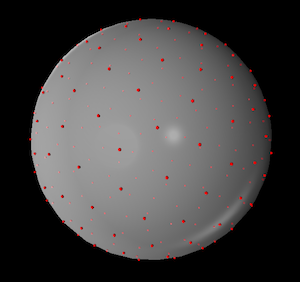
\includegraphics{images/screen_shot_1b.png}
\caption{}
\end{figure}

\textbf{Fig. 1}: \(N = 200\) excess charges in a spherical conductor.

The following figure shows an example using \(N = 1000\) excess charges.

\begin{figure}[htbp]
\centering
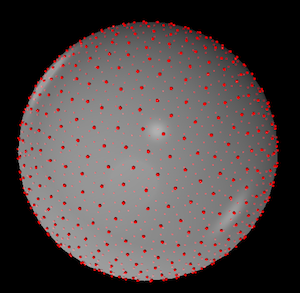
\includegraphics{images/screen_shot_2.png}
\caption{}
\end{figure}

\textbf{Fig. 2}: \(N = 1000\) excess charges in a spherical conductor.

\textbf{Exercise 3:}

Here is an example showing what the completed code for computing the
electric field at a point \(\vec{P}\) would like like if using
glowscript:

\begin{verbatim}
def computeEfield(P):
    ''' The COMPLETED function to compute the total electric field at point P, which is a 3D vector. '''
    
    global charges
    N = len(charges)
    
    # E_net will be computed from a summation, so it is first set to zero
    E_net = vec(0,0,0)
    
    # Loop through all charges in order to compute the net E field
    for charge in charges:
        r_vector = P - charge.pos # vector between charge & point P
        r = mag(r_vector)         # "r" is the magnitude of the r vector
        E = 1e-6 * K*q/r**2 * (r_vector/r) # The E field from this ONE charge
        E_net = E_net + E         # Computes the running sum, E_net
    return E_net # This sends the computed value back to the main loop
\end{verbatim}

The most important feature of this code is that instead of the
\textbf{\emph{nested}} loop, which was in the function to compute the
forces, this only includes a \textbf{\emph{single}} loop.

Note that depending on the programming language that is used to
implement this, it might be necessary to separately compute the vector
components for each (x, y, z) direction. (In glowscript, subtracting two
vectors results in the vector difference; and multiplying scalars by a
vector results in the appropriate new vector.)

Also note that in the example code (on the third from the last line),
multiplying by \texttt{1e-6} converts the electric field from units of
N/C to N/\(\mu\)C.

\textbf{Exercise 4:}

From Coulomb's Law, the electric field at a distance of \(r = 0.5\) m
away from a \(q=6\) \(\mu\)C charge is
\[E = \frac{kq}{r^2} = \frac{(8.99\times 10^9\textrm{ Nm$^2$/C$^2$})(5\times 10^{-6}\textrm{ C})}{(0.5\textrm{ m})^2}\]
which gives the result \(E = 1.798 \times 10^5\) N/C, or \(E = 0.1798\)
N/\(\mu\)C. (The sign of \(q\) is not relevant to the magnitude, \(E\).)

Running the simulation for a spherical conductor of radius \(R = 0.1\)
m, I get the same number \(E = 0.1798\) N/\(\mu\)C for the x-component
of \(\vec{E}\). This is good! (This was using a total of \(N=200\)
charges with total excess charge \(q=6\) \(\mu\)C.)

For the y and z components, the value is smaller by a factor of more
than 10,000, and as the simulation continues to run, these other
components are slowly converging toward zero.

\textbf{Exercise 5:}

From Coulomb's Law, the electric field at a distance of \(r = 0.15\) m
away from a \(q=6\) \(\mu\)C charge is
\[E = \frac{kq}{r^2} = \frac{(8.99\times 10^9\textrm{ Nm$^2$/C$^2$})(5\times 10^{-6}\textrm{ C})}{(0.15\textrm{ m})^2}\]
which gives the result \(E = 1.998 \times 10^6\) N/C, or \(E = 1.998\)
N/\(\mu\)C.

Running the simulation, I get \(E = 1.995\) N/\(\mu\)C for the
x-component of \(\vec{E}\), so the numbers differ by about 1.5\%. From
Gauss's Law, the two numbers should be the same. This slight difference
is due to the finite number of charges. When we get close to the
surface, the \(E\)-field will be somewhat irregular -- being influenced
by the precise positions of the individual charges, which results from
the charges' random initial positions.

\textbf{Exercise 6:}

When \textbf{\emph{inside}} of the conductor, the \(E\)-field starts out
large and fluctuates greatly for the first several time steps -- because
there is excess charge that is passing by the point of observation --
but once the charges get onto the surface and approach equilibrium, the
\(E\) field decays away to a small value. It didn't take long to reach
\(E \approx 10^{-3}\) N/\(\mu\)C, which is a thousand times smaller than
the \(E\)-field that was observed outside of the conductor. The dynamics
of this equilibriation is shown in the plot below. Due to the finite
number of charges, the \(E\)-field won't be exactly zero, but it will be
much smaller than the values that were observed outside of the
conductor.

\begin{figure}[htbp]
\centering
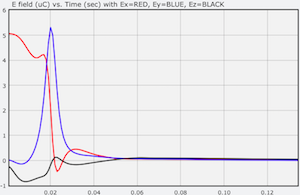
\includegraphics{images/EFieldInsideSphere.png}
\caption{}
\end{figure}

\textbf{Fig. 3}: Plot of each of the three components of \(\vec{E}\)
versus time for \(R=0.1\) m and \(r=0.05\) m. Within \(t=0.1\) seconds,
the electric field has become essentially zero.

\textbf{Exercise 7:}

The following figure shows the resulting configuration of \(N=8\) excess
charges in a conducting cube.

\begin{figure}[htbp]
\centering
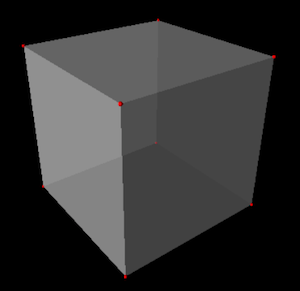
\includegraphics{images/cube_8.png}
\caption{}
\end{figure}

\textbf{Fig. 4}: \(N = 8\) excess charges in a cubical conductor. The 8
charges have ended up on the 8 corners of the cube.

The 8 charges push apart from one another and end up on the 8 corners of
the cube. This makes sense, because the charges go to the corners in
order to get as far away from each other as possible. (This minimizes
the energy of the system.) However, due to the random initial positions
of the charges, sometimes a charge gets ``stuck'' in the middle of an
edge, or in the middle of a surface, as shown below.

\begin{figure}[htbp]
\centering
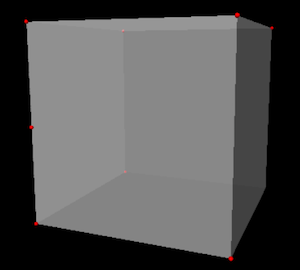
\includegraphics{images/cube_8_edge.png}
\caption{}
\end{figure}

\textbf{Fig. 5}: \(N = 8\) excess charges in a cubical conductor. One of
the 8 charges got stuck on the left edge, leaving one corner without a
charge (bottom-right-back).

\begin{figure}[htbp]
\centering
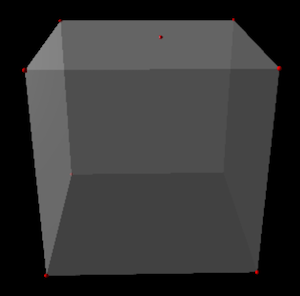
\includegraphics{images/cube_8_surface.png}
\caption{}
\end{figure}

\textbf{Fig. 6}: \(N = 8\) excess charges in a cubical conductor. One of
the 8 charges got stuck on the top surface, leaving one corner without a
charge (bottom-right-back).

\textbf{Exercise 8:}

The following figure shows the resulting configuration of \(N=20\)
excess charges in a conducting cube.

\begin{figure}[htbp]
\centering
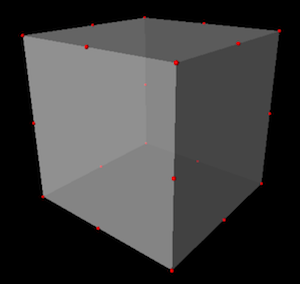
\includegraphics{images/cube_20.png}
\caption{}
\end{figure}

\textbf{Fig. 7}: \(N = 20\) excess charges in a cubical conductor. The
charges end up on each corner (8 charges) and in the middle of each edge
(12 charges). This is the configuration that minimizes the energy of the
system.

With \(N=20\) charges, it is common to end up with two charges that are
``stuck'' along an edge together, leaving another edge without a charge.

\begin{figure}[htbp]
\centering
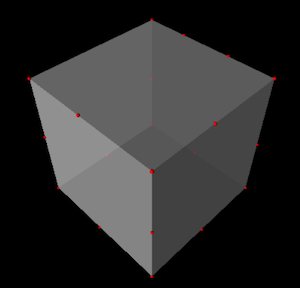
\includegraphics{images/cube_20_edge.png}
\caption{}
\end{figure}

\textbf{Fig. 8}: \(N = 20\) excess charges in a cubical conductor. Two
charges are stuck along one edge (back right) leaving another edge with
no charges (back left).

\textbf{Exercise 9:}

\begin{figure}[htbp]
\centering
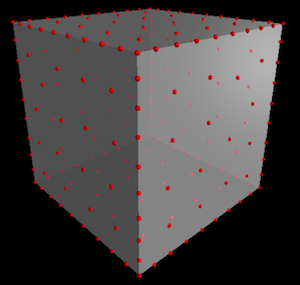
\includegraphics{images/cube_200.png}
\caption{}
\end{figure}

\textbf{Fig. 9}: \(N = 200\) excess charges in a cubical conductor. With
\(N = 200\) charges we can clearly see that the charges are closer to
one another along the edges, and they are farther apart from one another
on the surfaces.

\textbf{Exercise 10:}

This is the same as Exercise 4, but with a cube instead of a sphere. The
\(E\)-field from a point charge is \(E = 0.1798\) N/\(\mu\)C. (See the
solution for Exercise 4.) Running the simulation for a cubical conductor
of edge length \(L = 0.1\) m, I get the almost exactly the same number
\(E = 0.17973\) N/\(\mu\)C for the x-component of \(\vec{E}\). (This was
using a total of \(N=200\) charges with total excess charge \(q=6\)
\(\mu\)C.) So when we are far from the cube, the cube looks like a point
charge!

For the y and z components, the value is smaller by a factor of more
than 10,000, and as the simulation continues to run, these other
components are slowly converging toward zero.

\textbf{Exercise 11:}

At a distance of \(r=0.1\) m from a charge of \(q = 6\) \(\mu\)C, the
electric field would be
\[E = \frac{kq}{r^2} = \frac{(8.99\times 10^9\textrm{ Nm$^2$/C$^2$})(5\times 10^{-6}\textrm{ C})}{(0.1\textrm{ m})^2}\]
which gives the result \(E = 4.495\) N/\(\mu\)C.

I executed the simulation to compute the electric field at a distance of
\(x = 0.1\) m from the center of a cube of edge length \(L=0.1\) m. From
the simulation, \(E = 3.611\) N/\(\mu\)C. This value is quite a bit less
than \(E = 4.495\) N/\(\mu\)C! (The other components were smaller by a
factor of 1000 or more.)

For a \emph{sphere}, the electric field outside of the conductor was the
same as the electric field due to a point charge at the origin. This is
\textbf{NOT} the case for a cube. The complex charge distribution on the
surface of the cube produces an electric field that cannot (to my
knowledge) be calculated analytically. This is because the cube lacks
the symmetry of the sphere.

\textbf{Exercise 12:}

The result for the electric field inside of the cube is just like it was
inside of the sphere. Inside the conducting cube, the \(E\)-field starts
out large and fluctuates greatly for the first several time steps --
because there is excess charge that is passing by the point of
observation -- but once the charges get onto the surface and approach
equilibrium, the \(E\) field decays away to a small value. Due to the
finite number of charges, the \(E\)-field won't be exactly zero, but it
will be much smaller than the values that were observed outside of the
conductor.

When looking at the E-field inside the conductor, there is one
difference that you might notice between the sphere and the cube. For
the cube, the E-field might not go to exactly zero. An example of this
is shown in the figure below. This is because charges can -- and will --
get ``stuck'' on a particular edge or surface of a cube (which does not
happen with a sphere). In an \emph{actual} cube, there are slight
irregularities in the geometry that will allow charges to ``escape''
from an edge/surface. In the model that we are using, the geometry of
the cube is perfect, so it is not possible to leave from an
edge/surface.

\begin{figure}[htbp]
\centering
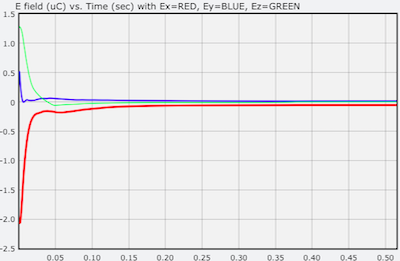
\includegraphics{images/InsideCube.png}
\caption{}
\end{figure}

\textbf{Fig. 10}: Plot of each of the three components of \(\vec{E}\)
versus time for a cube with edge length \(L=0.1\) m and \(r=0.01\) m.
The charges equilibriate quickly (within \(t=0.2\) seconds), but \(E_x\)
(red curve) goes to a small value that is not quite zero.

\subsection{Connections to Physics
Texts}\label{connections-to-physics-texts}

Any introductory physics textbook has a section on Gauss's Law and the
behavior of charges in a conductor.

\end{document}
